\documentclass[11pt,a4paper]{article}
\usepackage{fontspec}
\usepackage{amsmath,amssymb}
\usepackage{unicode-math}
\setmainfont{Latin Modern Roman}
\setmathfont{Latin Modern Math}
\usepackage{polyglossia}
\setdefaultlanguage[spelling=new]{german}
\usepackage[margin=2.3cm]{geometry}
\usepackage{booktabs,enumitem,array}
\usepackage[most]{tcolorbox}
\usepackage{tikz}
\usepackage[hidelinks]{hyperref}
\setlength{\parindent}{0pt}
\setlength{\parskip}{5pt}

% --- Notation ---
\newcommand{\ket}[1]{\lvert #1\rangle}
\newcommand{\bra}[1]{\langle #1\rvert}
\newcommand{\up}{{\uparrow}}
\newcommand{\dn}{{\downarrow}}
\newcommand{\Hbar}{\bar H}

% --- Kästen ---
\newtcolorbox{merk}[1][]{colback=green!4,colframe=green!45!black,fonttitle=\bfseries,title=Merke,#1}
\newtcolorbox{rechnung}[1][]{colback=gray!5,colframe=gray!55,fonttitle=\bfseries,title=Zwischenrechnung,#1}
\newtcolorbox{falle}[1][]{colback=red!4,colframe=red!60!black,fonttitle=\bfseries,title=Achtung,#1}
\newtcolorbox{warum}[1][]{colback=blue!4,colframe=blue!50!black,fonttitle=\bfseries,title=Warum?,#1}

\title{Lernskript: Das Heisenberg-Modell und die Hamilton-Matrix\\[2pt]\large Begleitend zu Übungsblatt 4 und Skript Bulla, Kap.~2}
\author{}
\date{Stand: 25.\,11.\,2026}

\begin{document}
\maketitle
\vspace{-1.5em}

\noindent\textbf{Quelle:} Vorlesungsskript „Computational Many-Body Physics“, apl.~Prof.~Dr.~R.~Bulla, SS~2022, Kapitel~2 (im Lesepaket S.~3–12). Seitenangaben „Skript S.~$k$“ meinen die Seitennummer innerhalb von Kapitel~2.

\noindent\textbf{Konventionen (wie im Skript):}\\ $\hbar=1$, Spin-$\tfrac12$, $J>0$ ferromagnetisch, $J<0$ antiferromagnetisch,
\[
H = -\sum_{i<j}\sum_{\alpha=x,y,z} J^\alpha_{ij}\,S^\alpha_i S^\alpha_j .
\]

\tableofcontents

%======================================================================
\section{Aufwärmen: ein einzelner Spin-\texorpdfstring{$\tfrac12$}{1/2}}

Ein Spin-$\tfrac12$ hat zwei Zustände, $\ket{\up}$ und $\ket{\dn}$. Sie sind Eigenzustände von $S^z$ (Skript S.~2):
\[
S^z\ket{\up} = +\tfrac12\ket{\up},\qquad S^z\ket{\dn} = -\tfrac12\ket{\dn}.
\]

Die \emph{Leiteroperatoren} (\emph{ladder operators}) sind
\[
S^\pm = S^x \pm i\,S^y .
\]
Sie klappen einen Spin um oder geben null:
\[
S^+\ket{\dn} = \ket{\up},\quad S^+\ket{\up} = 0,\qquad S^-\ket{\up} = \ket{\dn},\quad S^-\ket{\dn} = 0 .
\]

\begin{merk}
Anschaulich: $S^+$ hebt an, $S^-$ senkt ab. Was schon oben ist, kann nicht höher; was unten ist, nicht tiefer.
\end{merk}

%======================================================================
\section{Aufgabe 1a: \texorpdfstring{$H$}{H} mit \texorpdfstring{$S^\pm$}{S+-} umschreiben}

\textbf{Aufgabe} (Blatt~4, 1a): Schreibe $H = -\sum_{i<j,\alpha} J^\alpha_{ij}S^\alpha_iS^\alpha_j$ mit $S^\pm_i$ und $S^z_i$ um.

\subsection{Schritt 1: \texorpdfstring{$S^x$}{Sx} und \texorpdfstring{$S^y$}{Sy} durch \texorpdfstring{$S^\pm$}{S+-} ausdrücken}

Ausgangspunkt sind die beiden Definitionen
\[
\text{(I)}\quad S^+_i = S^x_i + i\,S^y_i,\qquad \text{(II)}\quad S^-_i = S^x_i - i\,S^y_i .
\]

\begin{rechnung}
(I) + (II):\quad $S^+_i + S^-_i = 2S^x_i$ \quad$\Rightarrow$\quad $S^x_i = \tfrac12\big(S^+_i + S^-_i\big)$

(I) $-$ (II):\quad $S^+_i - S^-_i = 2i\,S^y_i$ \quad$\Rightarrow$\quad $S^y_i = \dfrac{1}{2i}\big(S^+_i - S^-_i\big) = -\dfrac{i}{2}\big(S^+_i - S^-_i\big)$
\end{rechnung}

\begin{falle}
$\dfrac1i = -i$, \emph{nicht} $+i$. (Erweitern mit $i$: $\tfrac1i = \tfrac{i}{i^2} = \tfrac{i}{-1}$.) \\
Typischer Fehler: $S^y_i = +\tfrac{i}{2}(S^+_i - S^-_i)$. Im Produkt $S^y_iS^y_j$ fällt der Fehler zufällig nicht auf, weil $(\pm\tfrac i2)^2 = -\tfrac14$; die Formel für $S^y$ allein bleibt aber falsch.
\end{falle}

\subsection{Schritt 2: Produkte ausmultiplizieren}

\textbf{x-Link:}
\begin{rechnung}
\[
S^x_iS^x_j = \tfrac12\big(S^+_i + S^-_i\big)\cdot\tfrac12\big(S^+_j + S^-_j\big)
= \tfrac14\big(S^+_iS^+_j + S^+_iS^-_j + S^-_iS^+_j + S^-_iS^-_j\big)
\]
\end{rechnung}

\textbf{y-Link:} Zuerst die Vorfaktoren, dann die Klammern.
\begin{rechnung}
Vorfaktor:\quad $\dfrac{1}{2i}\cdot\dfrac{1}{2i} = \dfrac{1}{4\,i^2} = -\dfrac14$

Klammern:\quad $(S^+_i - S^-_i)(S^+_j - S^-_j) = S^+_iS^+_j - S^+_iS^-_j - S^-_iS^+_j + S^-_iS^-_j$
\[
\Rightarrow\quad S^y_iS^y_j = -\tfrac14\big(S^+_iS^+_j - S^+_iS^-_j - S^-_iS^+_j + S^-_iS^-_j\big)
\]
\end{rechnung}

\begin{falle}
Bei Produkten multiplizieren sich auch die Vorfaktoren: $\tfrac{1}{2i}\cdot\tfrac{1}{2i}$ enthält $i\cdot i = i^2 = -1$. Ein Vorfaktor $\tfrac{1}{4i}$ ist falsch.
\end{falle}

\textbf{z-Link} bleibt, wie er ist: $S^z_iS^z_j$ (immer ein \emph{Produkt} zweier Spins, nie eine Summe $S^z_1 + S^z_2 + \dots$ -- das wäre ein Magnetfeldterm).

\subsection{Schritt 3: Einsetzen, Klammerung beachten}

\[
H = -\sum_{i<j}\Big[\tfrac14 J^x_{ij}\big(S^+_iS^+_j + S^+_iS^-_j + S^-_iS^+_j + S^-_iS^-_j\big)
- \tfrac14 J^y_{ij}\big(S^+_iS^+_j - S^+_iS^-_j - S^-_iS^+_j + S^-_iS^-_j\big)
+ J^z_{ij}S^z_iS^z_j\Big]
\]

\begin{falle}
Das Minus vor $\sum$ gilt für \emph{alle} Terme. Darum die große eckige Klammer. Zieht man das Minus hinein, wechseln \emph{alle} Vorzeichen, auch beim z-Term: $-J^z_{ij}S^z_iS^z_j$. Die Summe $\sum_{i<j}$ bleibt stehen.
\end{falle}

\subsection{Schritt 4: Nach Operatoren sortieren}

Jedes Operatorprodukt kommt zweimal vor (aus dem x- und aus dem y-Link). Die Vorfaktoren werden zusammengefasst wie $3a + 5a = 8a$:

\begin{center}
\begin{tabular}{@{}lccc@{}}
\toprule
Operator & aus x-Link & aus y-Link & zusammen \\
\midrule
$S^+_iS^+_j$, $S^-_iS^-_j$ & $+\tfrac14J^x_{ij}$ & $-\tfrac14J^y_{ij}$ & $\tfrac14\big(J^x_{ij} - J^y_{ij}\big)$ \\[3pt]
$S^+_iS^-_j$, $S^-_iS^+_j$ & $+\tfrac14J^x_{ij}$ & $(-\tfrac14)(-1)J^y_{ij} = +\tfrac14J^y_{ij}$ & $\tfrac14\big(J^x_{ij} + J^y_{ij}\big)$ \\
\bottomrule
\end{tabular}
\end{center}

\begin{tcolorbox}[colback=yellow!6,colframe=orange!70!black,fonttitle=\bfseries,title=Ergebnis 1a]
\[
H = -\sum_{i<j}\Big[\tfrac14\big(J^x_{ij} - J^y_{ij}\big)\big(S^+_iS^+_j + S^-_iS^-_j\big)
+ \tfrac14\big(J^x_{ij} + J^y_{ij}\big)\big(S^+_iS^-_j + S^-_iS^+_j\big)
+ J^z_{ij}\,S^z_iS^z_j\Big]
\]
\end{tcolorbox}

\begin{merk}
Merkhilfe für die Vorzeichen: \textbf{gleiche} Operatoren ($++$, $--$) bekommen $J^x - J^y$, \textbf{gemischte} ($+-$, $-+$) bekommen $J^x + J^y$.
\end{merk}

\textbf{Kontrolle mit dem isotropen Heisenberg-Modell} ($J^x=J^y=J^z=J$):
\[
H = -J\sum_{i<j}\Big[\tfrac12\big(S^+_iS^-_j + S^-_iS^+_j\big) + S^z_iS^z_j\Big]
\]
Das stimmt mit Skript S.~3 überein.

%======================================================================
\section{Warum sortiert man nach Operatoren?}

Mathematisch ist es nicht nötig: die unsortierte Form ist derselbe Operator. Man sortiert, weil man dann die Physik direkt sieht.

\begin{warum}
\begin{enumerate}[leftmargin=*,itemsep=3pt]
\item \textbf{Welche Prozesse gibt es?}
  \begin{itemize}
  \item $S^+_iS^-_j$, $S^-_iS^+_j$: ein Spin hoch, der andere runter -- die beiden \emph{tauschen}. $S^z_\text{tot}$ bleibt gleich.
  \item $S^+_iS^+_j$, $S^-_iS^-_j$: \emph{beide} kippen in dieselbe Richtung. $S^z_\text{tot}$ ändert sich um $\pm2$ (jeder Spin um $\pm1$).
  \end{itemize}
\item \textbf{Wann fällt ein Prozess weg?} Vor den Doppel-Flips steht $J^x - J^y$. Für $J^x = J^y$ (Heisenberg, XXZ) gibt es sie nicht mehr $\Rightarrow$ $S^z_\text{tot}$ ist erhalten $\Rightarrow$ Blockstruktur der Matrix (Skript Kap.~2.2, S.~11--12).
\item \textbf{Matrixelemente direkt ablesen:} In der Basis $\ket n$ liefert jeder Term null oder genau einen Basiszustand:
\begin{align*}
\text{Paar antiparallel (tauschen):}&\quad -\tfrac14\big(J^x_{ij} + J^y_{ij}\big)\\
\text{Paar parallel (beide kippen):}&\quad -\tfrac14\big(J^x_{ij} - J^y_{ij}\big)
\end{align*}
Das ist dieselbe Idee wie das Vorzeichen $s$ beim y-Link im Skript (S.~8): $s=+1$ für antiparallele, $s=-1$ für parallele Spins.
\end{enumerate}
\end{warum}

Im Programm sortiert man \emph{nicht}: dort werden x- und y-Link getrennt behandelt und das Vorzeichen $s$ erledigt die Arbeit. Sortieren ist ein Werkzeug fürs Verstehen und Von-Hand-Rechnen.

%======================================================================
\section{Welche Basis wählt man -- und warum?}

Um $H$ als Matrix zu schreiben, braucht man eine Basis: $(\Hbar)_{mn} = \bra m H\ket n$. Im Skript (S.~2) ist das die \emph{Produktbasis} aus $S^z$-Eigenzuständen, z.\,B.\ für $N=3$
\[
\ket n = \ket{z_1}\otimes\ket{z_2}\otimes\ket{z_3},\qquad z_i\in\{0,1\},\qquad n = \sum_i z_i\,2^{\,i-1}.
\]

\subsection{Was jede Basis erfüllen muss}
\begin{itemize}[itemsep=2pt]
\item \textbf{vollständig}: $\sum_n\ket n\bra n = \mathbf 1$, sonst ist die Matrix nicht derselbe Operator wie $H$;
\item \textbf{orthonormiert}: $\langle m|n\rangle = \delta_{mn}$, sonst ist das Eigenwertproblem nicht einfach $\Hbar\vec\psi = E\vec\psi$.
\end{itemize}
Das gilt für \emph{jede} brauchbare Basis. Die Eigenwerte (Energien) hängen von der Wahl nicht ab, nur die Form der Matrix.

\subsection{Nach welchen Kriterien wählt man?}
\begin{warum}
\begin{enumerate}[leftmargin=*,itemsep=3pt]
\item \textbf{Einfach zu bauen:} Jeder Basiszustand ist eine Liste von Bits; $n$ ist eine Zahl. Das passt direkt in eine Schleife im Programm (Skript S.~9).
\item \textbf{$H$ wirkt einfach:} $S^z$ gibt nur eine Zahl $\pm\tfrac12$, $S^\pm$ macht aus einem Basiszustand genau einen anderen oder null. Jeder Link liefert pro Spalte höchstens ein Element $\Rightarrow$ dünn besetzte Matrix.
\item \textbf{Symmetrien sichtbar:} $S^z_\text{tot}$ ist in dieser Basis diagonal. Ist es erhalten (Heisenberg, XXZ), zerfällt $\Hbar$ in Blöcke (Skript S.~11--12).
\item \textbf{Passend zur Physik:} Je mehr $H$ zur Basis „passt“, desto näher ist $\Hbar$ an diagonal. Im Extremfall sind die Basiszustände schon die Eigenzustände.
\end{enumerate}
\end{warum}

\subsection{Die Basis für Blatt 4: \texorpdfstring{$2^N = 8$}{2\^N = 8} Zustände}

$2^N$ ist nicht die Basis selbst, sondern ihre \emph{Größe}: jeder der $N$ Spins hat 2 Möglichkeiten, also $2^3 = 8$ Basiszustände und eine $8\times8$-Matrix. Die Basis sind die 8 Zustände selbst, sortiert nach ihrem Label $n$:

\begin{center}
\begin{tabular}{@{}cccc@{}}
\toprule
$n$ & $[z_3z_2z_1]_2$ & Ket (Platz 1\,2\,3) & $S^z_\text{tot}$\\
\midrule
0 & 000 & $\ket{\dn\dn\dn}$ & $-\tfrac32$\\
1 & 001 & $\ket{\up\dn\dn}$ & $-\tfrac12$\\
2 & 010 & $\ket{\dn\up\dn}$ & $-\tfrac12$\\
3 & 011 & $\ket{\up\up\dn}$ & $+\tfrac12$\\
4 & 100 & $\ket{\dn\dn\up}$ & $-\tfrac12$\\
5 & 101 & $\ket{\up\dn\up}$ & $+\tfrac12$\\
6 & 110 & $\ket{\dn\up\up}$ & $+\tfrac12$\\
7 & 111 & $\ket{\up\up\up}$ & $+\tfrac32$\\
\bottomrule
\end{tabular}
\end{center}

\begin{falle}
Lesefalle: Im Ket steht Platz~1 \emph{links}, in der Binärzahl \emph{rechts}. $\ket{\up\dn\dn}$ ist $n=1$, nicht $n=4$.
\end{falle}

Das Matrixelement $(\Hbar)_{mn} = \bra m H\ket n$ steht in \textbf{Zeile $m$, Spalte $n$}. Man wendet $H$ auf den Spaltenzustand $\ket n$ an und liest ab, wie viel von $\ket m$ herauskommt.

\subsection{Spins als Bits: die Nummerierung}

\begin{itemize}[itemsep=2pt]
\item \textbf{1 Spin = 1 Bit:} $\up\leftrightarrow 1$, $\dn\leftrightarrow 0$.
\item \textbf{$N$ Spins = Register mit $N$ Bits:} jedes Bitmuster ist ein Basiszustand; $N$ Bits haben $2^N$ Muster. (Ein Byte: $2^8=256$ Muster $\Rightarrow$ 8 Spins hätten eine $256\times256$-Matrix.)
\item Die Nummer $n$ ist der Wert der Binärzahl $[z_N\dots z_1]_2$. Platz~1 ist das \emph{niedrigste} Bit (rechts).
\end{itemize}

\begin{falle}
Die Binärzahl ist \emph{keine eigene Basis}, sondern nur die Hausnummer der Produktzustände. Von Hand und im Programm ist es dieselbe Basis. \\
Begriff: „duale Basis“ heißt in der linearen Algebra etwas anderes (Basis des Dualraums, die Bras $\bra n$). Besser: „Binärdarstellung“ oder „Nummerierung im Dualsystem“.
\end{falle}

\textbf{Alle Zustände aufzählen -- binär zählen (Kilometer\-zähler-Muster).}\\ Man zählt $n=0,1,\dots,2^N-1$ hoch. Platz $i$ klappt dabei alle $2^{\,i-1}$ Schritte um:
\[
\text{Platz 1: } \dn\up\dn\up\dn\up\dn\up,\qquad
\text{Platz 2: } \dn\dn\up\up\dn\dn\up\up,\qquad
\text{Platz 3: } \dn\dn\dn\dn\up\up\up\up .
\]
Die drei Spalten nebeneinander ergeben die Tabelle oben -- vollständig, ohne Doppelte. Rückwärts: $n = \sum_i z_i\,2^{\,i-1}$ (jedes $\up$ mit seinem Stellenwert $1,2,4,\dots$ addieren).

\textbf{Warum $8\times8$?} Eine Zeile und eine Spalte pro Basiszustand: $n$ (Spalte) $=$ worauf $H$ wirkt, $m$ (Zeile) $=$ was herauskommt. $H$ bildet einen Vektor mit 8 Koeffizienten auf einen mit 8 Koeffizienten ab: $\vec\psi\,' = \Hbar\,\vec\psi$. Allgemein $2^N\times2^N$.

\textbf{Warum ab 0 zählen?}
\begin{enumerate}[itemsep=1pt]
\item $n=\sum_i z_i2^{\,i-1}$ gibt für $\ket{\dn\dn\dn}$ automatisch $0$, für $\ket{\up\up\up}$ den Wert $7$ -- die Nummer ist der Wert der Binärzahl.
\item Die Flip-Regel $l = n + (1-2z_p)2^{p-1} + (1-2z_q)2^{q-1}$ funktioniert direkt mit dieser Nummerie\-rung.
\item Python zählt ab 0: später ist $n$ direkt der Matrixindex.
\end{enumerate}
Ab 1 zu zählen ist mathematisch gleichwertig, verlangt aber überall „Index $=n+1$“ (so z.\,B.\ in Julia). Hauptsache einheitlich für Zeilen und Spalten.

\begin{warum}
\emph{(Über das Skript hinaus)} Ein klassisches Register speichert zu jedem Zeitpunkt \emph{ein} Bitmuster: 3 Bits $=$ 3 Zahlen (0 oder 1). Ein Quantenzustand kann eine Überlagerung \emph{aller} $2^N$ Muster sein, $\ket\psi = \sum_n \psi_n\ket n$: 3 Spins $=$ 8 komplexe Zahlen. Daher die große Dimension -- dieselbe Idee wie beim Qubit.
\end{warum}

\subsection{Alternativen \emph{(über das Skript hinaus)}}
\begin{itemize}[itemsep=2pt]
\item \textbf{$S^x$-Basis:} sinnvoll, wenn $H$ vor allem $S^xS^x$ oder ein Feld in $x$-Richtung enthält.
\item \textbf{Gesamtspin-Basis} (Eigenzustände von $\vec S_\text{tot}^{\,2}$ und $S^z_\text{tot}$, z.\,B.\ Singulett/Triplett): Für das Heisenberg-Modell mit $N=2$ ist $\Hbar$ darin sofort diagonal. Für großes $N$ sind diese Zustände aber mühsam zu konstruieren -- darum nimmt man für die exakte Diagonalisierung die Produktbasis und lässt den Computer diagonalisieren.
\end{itemize}

\begin{merk}
Die Basis ist ein Werkzeug, keine Physik: Energien hängen nicht von ihr ab. Man wählt die, in der $H$ am einfachsten wirkt und die man leicht programmieren kann -- für Spinmodelle die $S^z$-Produktbasis.
\end{merk}

%======================================================================
\section{Hilbertraum und Ortsraum -- was heißt „Dimension“?}

\subsection{Dimension = Anzahl der Basiszustände}

Die Dimension des Hilbertraums ist die Anzahl der Basiszustände, die man mindestens braucht, um \emph{jeden} Zustand darzustellen. Gleichwertig: die Anzahl der Koeffizienten $\psi_n$ in
\[
\ket\psi = \sum_{n=0}^{2^N-1}\psi_n\,\ket n
\qquad\widehat{=}\qquad
\vec\psi = (\psi_0,\psi_1,\dots,\psi_{2^N-1})^T\in\mathbb C^{2^N}.
\]

\begin{center}
\begin{tabular}{@{}lll@{}}
\toprule
Spins & Basiszustände & Dimension\\
\midrule
$N=1$ & $\ket\up,\ \ket\dn$ & 2\\
$N=2$ & $\ket{\dn\dn},\ \ket{\up\dn},\ \ket{\dn\up},\ \ket{\up\up}$ & 4\\
$N=3$ & $\ket 0,\dots,\ket 7$ & 8\\
$N$ & $\ket 0,\dots,\ket{2^N-1}$ & $2^N$\\
\bottomrule
\end{tabular}
\end{center}

Ein einzelner Zustand kann viele Koeffizienten null haben (z.\,B.\ $\ket{\up\dn\up}$: nur $\psi_5 = 1$). Die Dimension sagt, wie viele Bausteine man bereithalten muss, damit \emph{jeder} Zustand darstellbar ist.

\subsection{Die Basisvektoren als Spalten}

In der Basis aus Abschnitt~4 ist jeder Basiszustand ein Einheitsvektor im $\mathbb C^8$:
\[
\ket 0 = (1,0,0,0,0,0,0,0)^T,\quad \ket 1 = (0,1,0,0,0,0,0,0)^T,\quad\dots,\quad \ket 7 = (0,0,0,0,0,0,0,1)^T .
\]
Diese Vektoren leben im Hilbertraum $\mathbb C^8$, nicht im Ortsraum. Jeder hat seine 1 an einer anderen Stelle $\Rightarrow$ die 8 Vektoren sind linear unabhängig, wie $\vec e_x,\vec e_y,\vec e_z$ im $\mathbb R^3$.

\subsection{Zwei verschiedene Räume}

\begin{center}
\begin{tabular}{@{}p{3cm}p{5.2cm}p{5.6cm}@{}}
\toprule
& Ortsraum & Hilbertraum\\
\midrule
Dimension & 3 & $2^N$ (hier 8)\\
Koordinaten & reell, $(x,y,z)$ & komplex, $\psi_0,\dots,\psi_7$\\
Was lebt dort? & die Spins (Ecken des Dreiecks), die gezeichneten Pfeile & die Zustände $\ket\psi$\\
Achsen & Raumrichtungen & die Basiszustände $\ket n$\\
\bottomrule
\end{tabular}
\end{center}

\begin{falle}
Die Pfeile, die wir für Spins zeichnen, sind ein \emph{Bild}, nicht der Zustandsvektor. 8 Vektoren im 3D-Ortsraum wären linear abhängig -- die 8 Zustandsvektoren leben aber im $\mathbb C^8$, nicht im Ortsraum.
\end{falle}

\subsection{Antiparallel im Raum, orthogonal im Hilbertraum}

Schon bei \emph{einem} Spin sieht man den Unterschied:
\[
\ket\up = \begin{pmatrix}1\\0\end{pmatrix},\qquad \ket\dn = \begin{pmatrix}0\\1\end{pmatrix},\qquad \langle\up|\dn\rangle = 0 .
\]
Als Raumpfeile zeigen $\up$ und $\dn$ entgegengesetzt ($180^\circ$) -- als Raumvektoren wären sie linear abhängig. Als Zustände sind sie orthogonal ($90^\circ$). \textbf{Der Winkel halbiert sich.}

\subsection{Die Bloch-Kugel \emph{(über das Skript hinaus)}}

Jeder Zustand eines einzelnen Spins lässt sich (bis auf eine unwichtige Gesamtphase) schreiben als
\[
\boxed{\ket\psi = \cos\tfrac\theta2\,\ket\up + e^{i\varphi}\sin\tfrac\theta2\,\ket\dn},\qquad 0\le\theta\le\pi,\quad 0\le\varphi<2\pi .
\]
Die beiden Winkel $(\theta,\varphi)$ legen einen Punkt auf einer Kugel fest -- der \emph{Bloch-Kugel}. Achtung: Die Bloch-Kugel ist \emph{keine} Kugel im Ortsraum, sondern eine Landkarte aller Zustände eines Spins, also des Hilbertraums $\mathbb C^2$. Der Pfeil dorthin zeigt in die Richtung, in die der Spin im Mittel zeigt: $\langle\vec S\rangle = \tfrac12(\sin\theta\cos\varphi,\ \sin\theta\sin\varphi,\ \cos\theta)$.

\begin{center}
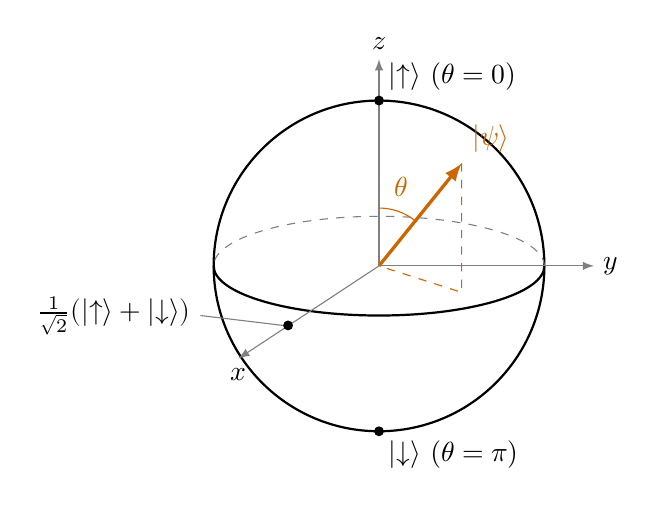
\begin{tikzpicture}[scale=2.1,>=latex]
  \draw[thick] (0,0) circle (1);
  \draw[dashed,gray] (1,0) arc (0:180:1 and 0.3);
  \draw[thick] (-1,0) arc (180:360:1 and 0.3);
  \draw[->,gray] (0,0) -- (0,1.25) node[above,black] {$z$};
  \draw[->,gray] (0,0) -- (-0.85,-0.56) node[below,black] {$x$};
  \draw[->,gray] (0,0) -- (1.3,0) node[right,black] {$y$};
  \fill (0,1) circle (0.03) node[above right] {$\ket\up$\ ($\theta=0$)};
  \fill (0,-1) circle (0.03) node[below right] {$\ket\dn$\ ($\theta=\pi$)};
  \fill (-0.55,-0.36) circle (0.03);
  \node[anchor=east] at (-1.08,-0.3) {$\tfrac1{\sqrt2}(\ket\up+\ket\dn)$};
  \draw[gray,thin] (-1.08,-0.3) -- (-0.58,-0.36);
  \draw[->,very thick,orange!80!black] (0,0) -- (0.5,0.62) node[above right] {$\ket\psi$};
  \draw[dashed,orange!80!black] (0.5,0.62) -- (0.5,-0.16) -- (0,0);
  \draw[orange!80!black] (0,0.35) arc (90:51:0.35);
  \node[orange!80!black] at (0.13,0.48) {$\theta$};
\end{tikzpicture}
\end{center}

\begin{itemize}[itemsep=2pt]
\item Nordpol $\theta=0$: $\ket\up$. Südpol $\theta=\pi$: $\ket\dn$. Gegenüberliegende Punkte $=$ orthogonale Zustände.
\item Äquator $\theta=\pi/2$: gleich große Überlagerung, z.\,B.\ $\tfrac1{\sqrt2}(\ket\up+\ket\dn)$ zeigt in $+x$-Richtung.
\item Das $\tfrac\theta2$ in der Formel ist genau die Winkelhalbierung: $180^\circ$ auf der Kugel $=$ $90^\circ$ im Hilbertraum.
\end{itemize}

\begin{merk}
Die Bloch-Kugel gilt nur für \emph{einen} Spin (Dimension 2). Schon für zwei Spins gibt es Zustände wie das Singulett, bei denen kein einzelner Spin einen Pfeil hat: $\langle\vec S_1\rangle = \langle\vec S_2\rangle = 0$. Dann hilft nur noch der Vektor $\vec\psi$ im $\mathbb C^{2^N}$ (Blatt 6: Verschränkung).
\end{merk}

\subsection{Warum die Dimension das Problem ist}

\begin{center}
\begin{tabular}{@{}rrl@{}}
\toprule
$N$ & $2^N$ & \\
\midrule
3 & 8 & Blatt 4, von Hand\\
10 & 1\,024 & Blatt 5, Laptop\\
20 & $\approx 10^6$ & nur als dünnbesetzte Matrix\\
40 & $\approx 10^{12}$ & Grenze der exakten Diagonalisierung\\
\bottomrule
\end{tabular}
\end{center}
Jeder Spin verdoppelt die Dimension; die volle Diagonalisierung kostet $\sim(2^N)^3$ (Skript S.~10). Daher Symmetrien (Blöcke) und später iterative Verfahren (Kap.~4.2).

%======================================================================
\section{Aufgabe 1b: Das Ising-Modell}

\textbf{Aufgabe} (Blatt~4, 1b): Stelle von Hand die $8\times8$-Matrix $\Hbar$ für das Ising-Modell auf, $J^\alpha_{ij} = J\,\delta_{\alpha z}$.

\subsection{Das Kronecker-Delta}

Das Kronecker-Delta ist ein „Schalter“:
\[
\delta_{\alpha z} = \begin{cases} 1 & \alpha = z\\ 0 & \alpha = x \text{ oder } y\end{cases}
\]
Für die drei Richtungen heißt das
\[
J^x_{ij} = J\,\delta_{xz} = 0,\qquad J^y_{ij} = J\,\delta_{yz} = 0,\qquad J^z_{ij} = J\,\delta_{zz} = J .
\]

\begin{merk}
Ising: nur die z-Kopplung ist eingeschaltet, für alle Paare gleich $J$. \\
Zum Vergleich Heisenberg (1c): $J^\alpha_{ij} = J$ ohne Delta -- alle drei Richtungen an.
\end{merk}

\subsection{Einsetzen in das Ergebnis von 1a}

Beide Vorfaktoren der $S^\pm$-Terme verschwinden: $J^x_{ij} - J^y_{ij} = 0$ und $J^x_{ij} + J^y_{ij} = 0$. Übrig bleibt nur der z-Term:

\begin{tcolorbox}[colback=yellow!6,colframe=orange!70!black,fonttitle=\bfseries,title=Hamiltonian des Ising-Modells (Drei-Platz-Cluster)]
\[
H_\text{Ising} = -J\sum_{i<j} S^z_iS^z_j = -J\big(S^z_1S^z_2 + S^z_1S^z_3 + S^z_2S^z_3\big)
\]
\end{tcolorbox}

\begin{falle}
\begin{itemize}[leftmargin=*,itemsep=2pt]
\item Der Faktor $\tfrac14$ gehört \emph{nur} zu den $S^\pm$-Termen (er stammt aus $S^x=\tfrac12(\dots)$ und $S^y=\tfrac1{2i}(\dots)$). Der z-Term wurde nie umgeschrieben und hat den Vorfaktor $J^z_{ij}$ \emph{ohne} $\tfrac14$. Falsch: $-\tfrac J4\,S^z_iS^z_j$.
\item Die Summe $\sum_{i<j}$ bleibt stehen: drei Paare $(12)$, $(13)$, $(23)$, nicht nur eines.
\end{itemize}
\end{falle}

Das $\tfrac14$ taucht trotzdem auf -- aber erst beim Anwenden auf einen Zustand: $S^z_iS^z_j$ liefert $\big(\pm\tfrac12\big)\big(\pm\tfrac12\big) = \pm\tfrac14$.

\subsection{Was man für die Matrixelemente braucht}

\begin{enumerate}[itemsep=2pt]
\item Eigenwerte eines Spins: $S^z\ket\up = +\tfrac12\ket\up$, \quad $S^z\ket\dn = -\tfrac12\ket\dn$.
\item $S^z_i$ wirkt nur auf Platz $i$; die anderen Spins bleiben unberührt.
\item Ein Paar liefert das Produkt der Eigenwerte:
\[
\up\up:\ \big(+\tfrac12\big)\big(+\tfrac12\big)=+\tfrac14,\qquad
\dn\dn:\ \big(-\tfrac12\big)\big(-\tfrac12\big)=+\tfrac14,\qquad
\up\dn,\ \dn\up:\ -\tfrac14 .
\]
\end{enumerate}

\begin{falle}
$S^z$ gibt für $\up$ und $\dn$ \emph{entgegengesetzte} Eigenwerte ($\pm\tfrac12$). Gleich ist nur das \emph{Produkt} eines Paares, wenn beide Spins gleich stehen -- egal ob beide oben oder beide unten.
\end{falle}

\subsection{Warum die Ising-Matrix diagonal ist}

$S^z_iS^z_j$ kippt keinen Spin, es multipliziert den Zustand nur mit einer Zahl: $H\ket n = E_n\ket n$. Mit der Orthonormalität $\langle m|n\rangle = \delta_{mn}$ folgt
\[
(\Hbar)_{mn} = \bra m H\ket n = E_n\,\langle m|n\rangle = E_n\,\delta_{mn} .
\]
Das ist dasselbe wie im Skript (S.~8): $\bra m J^z_{pq}S^z_pS^z_q\ket n = \tfrac14J^z_{pq}(2z_p-1)(2z_q-1)\,\delta_{mn}$.

\begin{merk}
Zwei Kronecker-Deltas, gleiches Symbol, andere Indizes: $\delta_{\alpha z}$ vergleicht \emph{Richtungen} (welche Kopplung an ist), $\delta_{mn}$ vergleicht \emph{Zustandsnummern} (wo in der Matrix ein Eintrag steht).
\end{merk}

\subsection{Die Diagonalelemente}

Rezept: drei Paare $(12),(13),(23)$ ansehen, Beiträge $\pm\tfrac14$ addieren, mit $-J$ multiplizieren.

\begin{rechnung}
$\ket 0 = \ket{\dn\dn\dn}$: \quad $+\tfrac14+\tfrac14+\tfrac14 = \tfrac34$ \quad$\Rightarrow$\quad $(\Hbar)_{00} = -J\cdot\tfrac34 = -\tfrac34J$

$\ket 1 = \ket{\up\dn\dn}$: \quad $(12)\ \up\dn: -\tfrac14,\ (13)\ \up\dn: -\tfrac14,\ (23)\ \dn\dn: +\tfrac14$ \quad Summe $-\tfrac14$
\[
(\Hbar)_{11} = -J\cdot\big(-\tfrac14\big) = +\tfrac14 J
\]
\end{rechnung}

\begin{falle}
Zwei Minuszeichen: das Vorzeichen jedes Paarbeitrags \emph{und} das $-J$ vor $H$. Minus mal Minus macht die Einträge der Zustände mit einem abweichenden Spin \emph{positiv}.
\end{falle}

\begin{tcolorbox}[colback=yellow!6,colframe=orange!70!black,fonttitle=\bfseries,title=Ergebnis 1b: Ising-Matrix]
\[
\Hbar_\text{Ising} = \frac J4\,\mathrm{diag}\big(-3,\ 1,\ 1,\ 1,\ 1,\ 1,\ 1,\ -3\big)
\qquad (n = 0,1,\dots,7)
\]
alle Spins parallel ($\ket{\dn\dn\dn}$, $\ket{\up\up\up}$): $-\tfrac34J$; \quad ein Spin weicht ab (die 6 übrigen): $+\tfrac14J$.
\end{tcolorbox}

\textbf{Zwei Proben:}
\begin{enumerate}[itemsep=2pt]
\item \emph{Alle Spins umdrehen} ändert kein Produkt $S^z_iS^z_j$ $\Rightarrow$ ein Zustand und sein Spiegelbild haben dieselbe Energie ($\ket1\leftrightarrow\ket6$, $\ket2\leftrightarrow\ket5$, $\ket3\leftrightarrow\ket4$, $\ket0\leftrightarrow\ket7$).
\item \emph{Spur $=0$}: jedes Paar steht über alle 8 Zustände gleich oft parallel wie antiparallel. $2\cdot(-\tfrac34) + 6\cdot\tfrac14 = 0$ \checkmark
\end{enumerate}

Da die Matrix diagonal ist, \emph{sind} die Diagonalelemente schon die Eigenenergien: $-\tfrac34J$ (2-fach), $+\tfrac14J$ (6-fach). Für $J>0$ sind die beiden voll ausgerichteten Zustände die Grundzustände.

%======================================================================
\section{Aufgabe 1c: Das Heisenberg-Modell (in Arbeit)}

\textbf{Aufgabe} (Blatt~4, 1c): $8\times8$-Matrix für das isotrope Heisenberg-Modell, $J^\alpha_{ij} = J$.

\subsection{Was man braucht}
\begin{enumerate}[itemsep=2pt]
\item Leiteroperatoren: $S^+\ket\dn = \ket\up,\ S^+\ket\up = 0,\quad S^-\ket\up = \ket\dn,\ S^-\ket\dn = 0$.
\item $S^z$-Eigenwerte und Paarbeiträge wie in 1b ($\pm\tfrac12$ bzw.\ $\pm\tfrac14$).
\item Hamiltonian aus Ergebnis 1a mit $J^x=J^y=J^z=J$:
\[
H_\text{Heis} = -J\sum_{i<j}\Big[\underbrace{S^z_iS^z_j}_{\text{wie Ising}} + \underbrace{\tfrac12\big(S^+_iS^-_j + S^-_iS^+_j\big)}_{\text{neu: Tausch}}\Big],
\qquad (i,j)\in\{(1,2),(1,3),(2,3)\}.
\]
\item $(\Hbar)_{mn} = \bra mH\ket n$: Spalte $n$ $=$ worauf $H$ wirkt, Zeile $m$ $=$ was herauskommt.
\end{enumerate}

\subsection{Die Regel aus 1b gilt nicht mehr}

Bei Ising war jeder Basiszustand ein Eigenzustand: $(\Hbar)_{mn} = E_n\delta_{mn}$. Beim Heisenberg-Modell macht der Tausch-Term aus $\ket n$ einen \emph{anderen} Zustand $\ket l$. Daher (Skript S.~7--8):
\[
\bra mH\ket n = \underbrace{E^{zz}_n\,\delta_{mn}}_{S^zS^z\text{-Teil: Diagonale}} \;+\; \underbrace{\sum_{\text{Tausch-Paare}} \big(-\tfrac J2\big)\,\delta_{ml}}_{\text{Tausch-Teil: Zeile } l}
\]

\begin{falle}
Die Diagonalelemente sind jetzt \emph{nicht} mehr die Energien. Für die Eigenwerte muss man die Matrix diagonalisieren. \\
Begriff: $\delta_{mn}$ ist das \emph{Kronecker}-Delta (diskrete Indizes, Wert 0 oder 1), nicht die Dirac-Delta-Distribution $\delta(x-x')$ für kontinuierliche Variablen.
\end{falle}

\subsection{Wie der Tausch-Term wirkt}

Für jedes Paar $(i,j)$:
\begin{itemize}[itemsep=2pt]
\item $S^+_iS^-_j$ wirkt nur, wenn $i$ \emph{unten} und $j$ \emph{oben} ist;
\item $S^-_iS^+_j$ wirkt nur, wenn $i$ \emph{oben} und $j$ \emph{unten} ist;
\item parallele Spins: beide Terme geben null.
\end{itemize}
Bei einem antiparallelen Paar überlebt genau einer: die beiden Spins \textbf{tauschen}. Beitrag: $-J\cdot\tfrac12 = -\tfrac J2$ in Zeile $l$.

\begin{rechnung}
$\ket 1 = \ket{\up\dn\dn}$, Diagonale aus 1b: $+\tfrac14J$.
\begin{center}
\begin{tabular}{@{}cccl@{}}
\toprule
Paar & Spins & parallel? & Tausch ergibt\\
\midrule
(12) & $\up\dn$ & nein & $\ket{\dn\up\dn} = \ket 2$\\
(13) & $\up\dn$ & nein & $\ket{\dn\dn\up} = \ket 4$ \quad ($0\cdot1+0\cdot2+1\cdot4 = 4$)\\
(23) & $\dn\dn$ & ja & --\\
\bottomrule
\end{tabular}
\end{center}
\[
H\ket1 = \tfrac14J\ket1 - \tfrac J2\ket2 - \tfrac J2\ket4
\quad\Rightarrow\quad
(\Hbar)_{11} = \tfrac14J,\quad (\Hbar)_{21} = (\Hbar)_{41} = -\tfrac J2 .
\]
\end{rechnung}

\subsection{Wie man \texorpdfstring{$H$}{H} auf einen Zustand anwendet: Summe heißt einzeln}

\begin{falle}
\textbf{Fehler:} Die Terme nacheinander anwenden -- also den zweiten Tausch auf das Ergebnis des ersten. Das wäre ein \emph{Produkt} von Operatoren (in Richtung $H^2$), nicht $H$.

\textbf{Richtig:} $H$ ist eine \emph{Summe}. Jeder Summand wirkt auf den \emph{ursprünglichen} Zustand, die Ergebnisse werden addiert (Linearität):
\[
(A+B+C)\ket\psi = A\ket\psi + B\ket\psi + C\ket\psi \qquad\text{nicht}\qquad C\big(B(A\ket\psi)\big).
\]
Das gilt auf jeder Ebene: für die drei Gruppen, für die drei Paare in jeder Gruppe und für die beiden Terme $S^+_iS^-_j + S^-_iS^+_j$. Das Ergebnis ist eine \emph{Linearkombination} von Basiszuständen.

\textbf{Merke:} Ein \emph{Plus} zwischen Operatoren: jeden einzeln auf denselben Zustand. Operatoren \emph{direkt nebeneinander} (z.\,B.\ $S^-_1S^+_2$): nacheinander, von rechts nach links.
\end{falle}

Übersichtlich wird es, wenn man $H$ in drei Gruppen schreibt:
\[
H = -J\Big[\underbrace{\textstyle\sum_{i<j}S^z_iS^z_j}_{\text{A}}
+ \underbrace{\tfrac12\big(S^+_1S^-_2 + S^+_1S^-_3 + S^+_2S^-_3\big)}_{\text{B}}
+ \underbrace{\tfrac12\big(S^-_1S^+_2 + S^-_1S^+_3 + S^-_2S^+_3\big)}_{\text{C}}\Big]
\]

\begin{rechnung}
$\ket1 = \ket{\up\dn\dn}$ (Platz 1 oben, Platz 2 und 3 unten):

\textbf{B:} jeder Term braucht $S^-$ auf Platz 2 oder 3, dort steht $\dn$ $\Rightarrow$ B gibt komplett $0$.

\textbf{C:} $S^-_1S^+_2\ket{\up\dn\dn} = \ket{\dn\up\dn} = \ket2$, \quad $S^-_1S^+_3\ket{\up\dn\dn} = \ket{\dn\dn\up} = \ket4$, \quad $S^-_2S^+_3$: $S^-$ auf $\dn$ $\Rightarrow 0$.
\[
H\ket1 = -J\Big[\underbrace{-\tfrac14\ket1}_{\text{A}} + \underbrace{0}_{\text{B}} + \underbrace{\tfrac12\ket2 + \tfrac12\ket4}_{\text{C}}\Big]
= \tfrac14J\ket1 - \tfrac J2\ket2 - \tfrac J2\ket4 .
\]

$\ket2 = \ket{\dn\up\dn}$: antiparallel sind $(12)$ und $(23)$, parallel ist $(13)$:
\[
H\ket2 = \tfrac14J\ket2 - \tfrac J2\ket1 - \tfrac J2\ket4 .
\]
\end{rechnung}

\begin{merk}
Pro antiparallelem Paar liefert \emph{genau einer} der beiden Terme (aus B oder aus C) den Tausch, der andere gibt null. Bei parallelen Paaren geben beide null. \\
\textbf{Probe:} Anzahl der Tausch-Terme in $H\ket n$ $=$ Anzahl der antiparallelen Paare in $\ket n$ (bei genau einem abweichenden Spin: zwei).
\end{merk}

\textbf{Spalte $n$ der Matrix $=$ Koeffizienten von $H\ket n$.} Zustände, die in $H\ket n$ nicht vorkommen, bekommen in Spalte $n$ eine 0. Beispiel: in $H\ket1$ kommt $\ket3$ nicht vor $\Rightarrow (\Hbar)_{31} = (\Hbar)_{13} = 0$.

\subsection{Muster, die Arbeit sparen}
\begin{enumerate}[itemsep=2pt]
\item \textbf{Diagonale} $=$ Ising-Diagonale aus 1b.
\item \textbf{Außerhalb} nur dort $\neq0$, wo sich $\ket m$ und $\ket n$ in genau zwei Spins unterscheiden, die in $\ket n$ antiparallel stehen.
\item \textbf{Symmetrisch}: $(\Hbar)_{mn} = (\Hbar)_{nm}$ ($H$ hermitesch und reell) -- obere Hälfte rechnen, spiegeln.
\item \textbf{Alle Tausch-Einträge gleich}: $-\tfrac J2$.
\item \textbf{Blöcke}: Ein Tausch ändert die Zahl der $\up$ nicht ($S^z_\text{tot}$ erhalten). Nur innerhalb dieser Gruppen gibt es Einträge außerhalb der Diagonale:
\[
\underbrace{\{\ket0\}}_{0\,\up}\qquad
\underbrace{\{\ket1,\ket2,\ket4\}}_{1\,\up}\qquad
\underbrace{\{\ket3,\ket5,\ket6\}}_{2\,\up}\qquad
\underbrace{\{\ket7\}}_{3\,\up}
\]
\end{enumerate}

\begin{falle}
Typische Fehler beim ersten Versuch:
\begin{itemize}[leftmargin=*,itemsep=1pt]
\item \emph{Lesefalle}: $\ket{\dn\dn\up}$ ist $n=4$, nicht $3$. Probe: ein Eintrag zwischen verschiedenen Gruppen (z.\,B.\ $(\Hbar)_{13}$) kann nicht sein.
\item Diagonale ist dieselbe wie bei Ising, also $+\tfrac14J$ auch für $\ket3,\ket5,\ket6$.
\item Jeder Tausch-Beitrag ist $-\tfrac J2$, nie $+\tfrac J2$.
\end{itemize}
\end{falle}

\subsection{Offen}
\begin{enumerate}[itemsep=1pt]
\item Spalten 3, 5, 6 genauso aufstellen (Gruppe $\{3,5,6\}$).
\item Liste korrigieren, die $8\times8$-Matrix aufschreiben.
\item Eigenwerte der beiden $3\times3$-Blöcke über $\det(\Hbar_\text{Block} - E\,\mathbf 1) = 0$.
\end{enumerate}

%======================================================================
\section{Aufgabe 1d: Modell d (in Arbeit)}

\textbf{Aufgabe} (Blatt~4, 1d): $J^x_{12} = J^y_{23} = J^z_{31} = J$, \emph{alle anderen} $J^\alpha_{ij} = 0$.

\subsection{Nur drei Links bleiben}

\begin{center}
\begin{tabular}{@{}cccc@{}}
\toprule
Paar & $J^x$ & $J^y$ & $J^z$\\
\midrule
(12) & $\boldsymbol J$ & 0 & 0\\
(23) & 0 & $\boldsymbol J$ & 0\\
(31) & 0 & 0 & $\boldsymbol J$\\
\bottomrule
\end{tabular}
\end{center}
Von 9 möglichen Links bleiben 3; alle Terme mit Kopplung 0 fallen weg. Jedes Paar hat eine \emph{andere} Richtung -- das Grundprinzip des Kitaev-Modells (Skript Kap.~2.1; Blatt~6).

\begin{center}
\begin{tabular}{@{}ll@{}}
\toprule
Ising (1b) & 3 Links, alle $z$\\
Heisenberg (1c) & alle 9 Links\\
Modell d & 3 Links, jedes Paar eine andere Richtung\\
\bottomrule
\end{tabular}
\end{center}

\subsection{Einsetzen in Ergebnis 1a}

\begin{rechnung}
\textbf{(12):} $\tfrac14(J-0)(S^+_1S^+_2+S^-_1S^-_2) + \tfrac14(J+0)(S^+_1S^-_2+S^-_1S^+_2)$

\textbf{(23):} $\tfrac14(0-J)(S^+_2S^+_3+S^-_2S^-_3) + \tfrac14(0+J)(S^+_2S^-_3+S^-_2S^+_3)$

\textbf{(31):} $J\,S^z_3S^z_1$
\[
H_d = -\Big[\tfrac J4\big(S^+_1S^+_2 + S^-_1S^-_2 + S^+_1S^-_2 + S^-_1S^+_2\big)
- \tfrac J4\big(S^+_2S^+_3 + S^-_2S^-_3\big) + \tfrac J4\big(S^+_2S^-_3 + S^-_2S^+_3\big)
+ J\,S^z_3S^z_1\Big]
\]
\end{rechnung}

\begin{falle}
Bei Paar (23) ist $J^x_{23} - J^y_{23} = 0 - J = -J$: die Doppel-Flips bekommen $-\tfrac J4$.
\end{falle}

\subsection{Zurück zur Link-Darstellung: 1a rückwärts}

Liest man die Ergebnisse aus 1a von rechts nach links,
\[
S^x_iS^x_j = \tfrac14\big(S^+_iS^+_j + S^+_iS^-_j + S^-_iS^+_j + S^-_iS^-_j\big),\qquad
S^y_iS^y_j = -\tfrac14\big(S^+_iS^+_j - S^+_iS^-_j - S^-_iS^+_j + S^-_iS^-_j\big),
\]
dann erkennt man in $H_d$:
\begin{itemize}[itemsep=2pt]
\item Paar (12): alle vier Terme mit $\tfrac J4$ $\Rightarrow$ $J\,S^x_1S^x_2$;
\item Paar (23): gleiche Operatoren mit $-\tfrac J4$, gemischte mit $+\tfrac J4$ $\Rightarrow$ $J\,S^y_2S^y_3$.
\end{itemize}
\begin{tcolorbox}[colback=yellow!6,colframe=orange!70!black,fonttitle=\bfseries,title=Hamiltonian Modell d]
\[
H_d = -J\big(S^x_1S^x_2 + S^y_2S^y_3 + S^z_3S^z_1\big)
\]
\end{tcolorbox}

\subsection{Woher die Link-Regeln kommen (Skript S.~6--8)}

Auf einen Basiszustand angewendet, gibt von den vier Termen in $S^x_1S^x_2$ \emph{genau einer} nicht null:
\begin{center}
\begin{tabular}{@{}lll@{}}
\toprule
Spins 1, 2 & überlebender Term & Ergebnis\\
\midrule
$\dn\dn$ & $S^+_1S^+_2$ & beide hoch\\
$\up\up$ & $S^-_1S^-_2$ & beide runter\\
$\up\dn$ & $S^-_1S^+_2$ & tauschen\\
$\dn\up$ & $S^+_1S^-_2$ & tauschen\\
\bottomrule
\end{tabular}
\end{center}
In jedem Fall werden \emph{beide} Spins gekippt, Vorfaktor $\tfrac14$.

\begin{merk}
\begin{itemize}[leftmargin=*,itemsep=2pt]
\item \textbf{x-Link:} $S^x_pS^x_q\ket n = \tfrac14\ket l$ -- kippt \emph{immer} beide Spins. Eintrag in $H$: $-\tfrac14J$.
\item \textbf{y-Link:} $S^y_pS^y_q\ket n = s\cdot\tfrac14\ket l$, $s=+1$ antiparallel, $s=-1$ parallel (das Minus der gleichen Operatoren). Eintrag in $H$: $-s\cdot\tfrac14J$.
\item \textbf{z-Link:} kippt nichts, Diagonale: $\pm\tfrac14$ wie bei Ising, mal $-J$.
\end{itemize}
Unterschied zu 1c: Der Tausch-Term wirkte nur auf antiparallele Paare. $S^x$ und $S^y$ kippen \emph{immer}.
\end{merk}

Folge: $H_d\ket n$ hat stets drei Terme -- einen Diagonalterm (z-Link), einen mit Spins 1, 2 gekippt (x-Link), einen mit Spins 2, 3 gekippt (y-Link). Man kann mit der $S^\pm$-Form oder mit den Link-Regeln rechnen; die $S^\pm$-Form hat nur mehr Terme, die null geben.

\subsection{Offen}
\begin{enumerate}[itemsep=1pt]
\item $H_d\ket0$ für $\ket{\dn\dn\dn}$: Auf $\ket{\dn\dn\dn}$ wirken nur Terme mit ausschließlich $S^+$.
\item Alle 8 Spalten, $8\times8$-Matrix.
\item Bleibt die Zahl der $\up$ erhalten? Was heißt das für die Blöcke?
\end{enumerate}

%======================================================================
\section[Exkurs: Determinante und Kommutator]{Exkurs: Determinante und Kommutator\\\large\emph{(über das Skript hinaus)}}

\textbf{Gemeinsam: beide sind antisymmetrisch.}
\begin{center}
\begin{tabular}{@{}lll@{}}
\toprule
& Kommutator & Determinante\\
\midrule
Vertauschen & $[A,B] = -[B,A]$ & zwei Zeilen tauschen: Vorzeichenwechsel\\
Gleiches doppelt & $[A,A] = 0$ & zwei gleiche Zeilen: $\det = 0$\\
Form & $AB - BA$ & $\det\begin{pmatrix}a&b\\c&d\end{pmatrix} = ad - bc$\\
Levi-Civita & $[S^i,S^j] = i\sum_k\varepsilon_{ijk}S^k$ & $\det(\vec a,\vec b,\vec c) = \sum_{ijk}\varepsilon_{ijk}a_ib_jc_k$\\
\bottomrule
\end{tabular}
\end{center}

\textbf{Unterschied:} Die Determinante macht aus \emph{einer} Matrix eine \emph{Zahl} (Volumen, invertierbar?). Der Kommutator macht aus \emph{zwei} Operatoren einen neuen \emph{Operator} (spielt die Reihenfolge eine Rolle?). Verbindung: $\operatorname{tr}[A,B] = 0 \Rightarrow \det e^{[A,B]} = 1$.

\begin{merk}
Wo beides in Blatt~4 vorkommt: $[H,S^z_\text{tot}]=0$ erklärt die Blöcke; $\det(\Hbar_\text{Block}-E\,\mathbf1)=0$ liefert die Eigenwerte eines Blocks von Hand.
\end{merk}

%======================================================================
\section{Methodenkarte}

\begin{center}
\begin{tabular}{@{}>{\raggedright\arraybackslash}p{3.2cm}>{\raggedright\arraybackslash}p{5.6cm}>{\raggedright\arraybackslash}p{5.2cm}@{}}
\toprule
Gebiet & Werkzeug & wo benutzt \\
\midrule
Komplexe Zahlen & $\tfrac1i = -i$, $i^2=-1$ & $S^y$ durch $S^\pm$, Vorfaktor $-\tfrac14$ \\
Lineare Algebra & Gleichungssystem (I)$\pm$(II) lösen & $S^x$, $S^y$ aus $S^\pm$ \\
Operatoralgebra & Ausmultiplizieren, Reihenfolge $i$ vor $j$ beibehalten & $S^\alpha_iS^\alpha_j$ in $S^\pm$ \\
Algebra & Ausklammern, nach Operatoren sortieren & Ergebnis 1a \\
Quantenmechanik & $S^\pm$ als Leiteroperatoren & Deutung: Tausch vs.\ Doppel-Flip \\
Notation & Kronecker-Delta $\delta_{\alpha z}$ als Schalter & Ising-Kopplungen in 1b \\
Lineare Algebra & Orthonormalität $\langle m|n\rangle=\delta_{mn}$ & Ising-Matrix diagonal \\
Kontrolle & Symmetrie (alle Spins umdrehen), Spur & Probe der Diagonale in 1b \\
Quantenmechanik & $S^\pm$ auf Paare: Tausch antiparalleler Spins & Einträge außerhalb der Diagonale in 1c \\
Symmetrie & Erhaltung von $S^z_\text{tot}$ $\Rightarrow$ Blöcke & Probe der Einträge in 1c \\
\bottomrule
\end{tabular}
\end{center}

%======================================================================
\section{Stand und nächste Schritte}

\textbf{Kann ich:}
\begin{itemize}[itemsep=1pt]
\item $S^x$, $S^y$ durch $S^\pm$ ausdrücken (mit $\tfrac1i=-i$)
\item Operatorprodukte ausmultiplizieren, Vorfaktor $\tfrac{1}{2i}\cdot\tfrac{1}{2i} = -\tfrac14$
\item nach Operatoren sortieren und Kopplungen zusammenfassen, Minus vor der Summe korrekt behandeln
\item Kronecker-Delta lesen und einsetzen; $H_\text{Ising} = -J\sum_{i<j}S^z_iS^z_j$ aufstellen
\item begründen, warum man die $S^z$-Produktbasis wählt
\item Spins als Bits verstehen, alle $2^N$ Zustände systematisch aufzählen, Nummerierung ab 0 begründen
\item Dimension des Hilbertraums erklären; Ortsraum und Hilbertraum unterscheiden; Bloch-Kugel für einen Spin
\item 1b: alle 8 Diagonalelemente der Ising-Matrix berechnen und mit Symmetrie und Spur prüfen
\item 1c: Tausch-Term auf Basiszustände anwenden, Paare $(i,j)$ durchgehen, Einträge $-\tfrac J2$ außer\-halb der Diagonale finden
\item 1d: Kopplungen einsetzen, $H_d$ aufstellen und zwischen $S^\pm$-Form und Link-Form umrechnen
\end{itemize}

\textbf{Noch üben:}
\begin{itemize}[itemsep=1pt]
\item Vorzeichen sauber verfolgen (Paarbeitrag und $-J$; Tausch immer $-\tfrac J2$)
\item Lesefalle beim Zuordnen der Nummern: $\ket{\dn\dn\up}=4$
\item Summen von Operatoren: jeden Summanden auf den \emph{ursprünglichen} Zustand anwenden, nicht nacheinander
\item Beim Ausschreiben Indizes und Vorzeichen prüfen (z.\,B.\ Paar (23) nicht von (12) abschreiben; Minus vor der Klammer)
\item Vorfaktoren nur dort ausklammern, wo sie hingehören; Summe nicht verlieren
\end{itemize}

\textbf{Als Nächstes -- Aufgabe 1c fertigstellen:}\\ $H\ket2$, Liste korrigieren (Probe: nur Einträge innerhalb der Gruppen gleicher $\up$-Zahl), $8\times8$-Matrix aufschreiben, Blöcke diagonalisieren.

\end{document}
